% Stanford University PhD thesis style -- modifications to the report style
% This is unofficial so you should always double check against the
% Registrar's office rules
% See http://library.stanford.edu/research/bibliography-management/latex-and-bibtex
% 
% Example of use below
% See the suthesis-2e.sty file for documentation
%
\documentclass{report}
\usepackage{suthesis-2e}
\usepackage[spanish]{babel}
\usepackage[utf8]{inputenc}
\usepackage[T1]{fontenc}
\usepackage{amsmath}
\usepackage{nccmath}
\usepackage{bm}
\usepackage{algorithm}
\usepackage[noend]{algpseudocode}
\usepackage{listingsutf8}
\usepackage{graphicx}
\usepackage{booktabs}
\usepackage{forest}
\usepackage[flushleft]{threeparttable}
\usepackage{cases}
\usepackage{subcaption}
\usepackage{float}
\usepackage{textcomp}
\usepackage{nicefrac}
\usepackage{booktabs,tabularx}
\usepackage{tikz}
\usetikzlibrary{trees}
\tikzstyle{every node}=[draw=black,thick,anchor=west, minimum height=2.5em]
\renewcommand{\tabularxcolumn}{m}
\newcommand{\tabitem}{~~\llap{\textbullet}~~}
\graphicspath{ {./} }

\definecolor{dkgreen}{rgb}{0,0.6,0}
\definecolor{gray}{rgb}{0.5,0.5,0.5}
\definecolor{mauve}{rgb}{0.58,0,0.82}

\lstset{frame=tb,
	language=C++,
	aboveskip=3mm,
	belowskip=3mm,
	showstringspaces=false,
	columns=flexible,
	basicstyle={\small\ttfamily},
	numbers=none,
	numberstyle=\tiny\color{gray},
	keywordstyle=\color{blue},
	commentstyle=\color{dkgreen},
	stringstyle=\color{mauve},
	breaklines=true,
	breakatwhitespace=true,
	tabsize=3,
	inputencoding=utf8/latin1,
	extendedchars=true,
	literate={á}{{\'a}}1 {ã}{{\~a}}1 {é}{{\'e}}1,
}


\dept{Computer Science}

\begin{document}
	\title{Documentación del sistema software \\
	de gestión de alumnos}
	\author{Grupo 6 \\
	Ortega León, Daniel\\
	Pérez Hernández, Julen\\
	Sevilla Molina, Ángel}
 
\beforepreface
\afterpreface

\chapter{Análisis de Requisitos}
\section{Análisis funcional}
En este apartado se incluye la parte funcional, estructural y el comportamiento de la aplicación. Para ello se hace uso de UML (Unified Modeling Language - Lenguaje Unificado de Modelado), un lenguaje gráfico para visualizar, especificar, construir y documentar un sistema.
\subsection{Identificación de actores del Sistema}
Un actor, en UML, es aquel agente externo (un usuario, un dispositivo hardware o incluso
otro sistema) que interactúa con el sistema.

Para este sistema se puede diferenciar el siguiente actor:
\begin{itemize}
	\item \textbf{Profesor:} Profesor: El profesor es el único actor del sistema, y es el que gestiona y opera con los datos de los alumnos. El profesor puede ser coordinador o ayudante.
\end{itemize}

\subsection{Datos}
El sistema debe permitir un registro histórico de alumnos que gestione la siguiente información: dni, nombre, apellidos, teléfono, e-mail, dirección postal, curso más alto matriculado, fecha de nacimiento, número de equipo, y si es líder o no del equipo.

\subsection{Requisitos}
\subsubsection{Requisitos funcionales}
Los requisitos funcionales son características que debe cumplir el sistema y que expresan la funcionalidad y/o el comportamiento específico que debe tener el sistema ante determinadas situaciones. Estos se codifican con las siglas \textit{RF}, seguidas de un guión y del número de requisito.
\begin{itemize}
	\item \textbf{RF-1:} El sistema permite que el profesor pueda añadir alumnos en la base de datos.
	\begin{itemize}
		\item \textbf{RF-1.1:} Todos los datos son obligatorios excepto el número de grupo y liderazgo.
	\end{itemize}
	\item \textbf{RF-2:} El sistema permite que el profesor pueda modificar la información de los alumnos ya registrados en la base de datos.
	\item \textbf{RF-3:} El sistema permite que el profesor pueda eliminar alumnos de la base de datos.
	\item \textbf{RF-4:} El sistema permite que el profesor pueda buscar alumnos.
	\begin{itemize}
		\item \textbf{RF-4.1:} La búsqueda de alumnos debe poder filtrarse a partir del dni, de los apellidos o del equipo al que pertenece.
		\item \textbf{RF-4.2:} La búsqueda debe devolver todas las coincidencias obtenidas.
	\end{itemize}
	\item \textbf{RF-5:} El sistema permite que el profesor pueda acceder a la información de uno o varios alumnos.
	\begin{itemize}
		\item \textbf{RF-5.1:} El profesor puede ordenar el mostrado en orden alfabético, por dni, o por curso más alto matriculado.
		\item \textbf{RF-5.2:} El orden puede ser ascendente o descendente.
	\end{itemize}
	\item \textbf{RF-6:} El sistema permite que el profesor pueda guardar los datos en un fichero de seguridad.
	\item \textbf{RF-7:} El sistema permite que el profesor pueda cargar los datos a partir de un fichero de seguridad.
	\item \textbf{RF-8:} El sistema debe incorporar un proceso de identificación mediante nombre y contraseña para que los profesores puedan hacer uso de las funcionalidades del sistema.
	\item \textbf{RF-9:} El sistema permite que el profesor coordinador pueda añadir ayudantes en el sistema, aportando nombre de profesor y contraseña.
\end{itemize}

\subsubsection{Requisitos no funcionales}
Los requisitos no funcionales son característicos del proceso de desarrollo, del servicio prestado o de cualquier otro aspecto del desarrollo, que debe cumplir el sistema y que indican las restricciones del mismo. Estos se codifican con las siglas \textit{RNF}, seguidas de un guión y del número de requisito.

\begin{itemize}
	\item \textbf{RNF-1:} El lenguaje de programación es C++.
	\item \textbf{RNF-2:} El lenguaje de documentación será Markdown.
	\item \textbf{RNF-3:} Si se hace uso de un IDE, éste será Eclipse.
	\item \textbf{RNF-4:} El proyecto se realizará haciendo uso del sistema de control de versiones Git y la plataforma GitHub para el almacenamiento del repositorio de forma remota.
	\item \textbf{RNF-5:} El historial de cambios queda guardado en las cuentas de Git por lo que la evaluación será incremental y no servirá subir los ficheros de un día para otro en Git.
	\item \textbf{RNF-6:} El sistema debe funcionar en Linux.
	\item \textbf{RNF-7:} El sistema deberá ser rápido ofreciendo los resultados de consulta en un tiempo inferior a dos segundos. Del mismo modo los procesos de actualización de un registro de la base de datos deben ser realizados en menos de un segundo.
	\item \textbf{RNF-7:} Se utilizará la metodología UML durante la fase de desarrollo.
	\item \textbf{RNF-8:} El sistema debe permitir almacenar información histórica.
	\item \textbf{RNF-9:} Se debe tener un alto control de errores, evitando que el profesor introduzca datos inconsistentes, y permitir al profesor la modificación o posibilidad de subsanar otros errores.
	\item \textbf{RNF-10:} El formato de salida de los listados de alumnos debe ser html o Markdown.
	\item \textbf{RNF-11:} El sistema solo puede admitir como máximo a 150 alumnos.
	\item \textbf{RNF-12:} Debe poderse cargar o guardar los datos del registro histórico de alumnos en ficheros binarios.
	\item \textbf{RNF-13:} Todos los datos de un alumno son necesarios, excepto el número de grupo y el liderazgo.
	\item \textbf{RNF-14:} Un alumno solo puede ser líder de un grupo si forma parte de un grupo.
	\item \textbf{RNF-15:} Como máximo puede haber un solo líder por grupo.
	\item \textbf{RNF-16:} En el mostrado, aquellos alumnos que sean líderes de un grupo deben verse remarcados.
	\item \textbf{RNF-17:} Los atributos identificadores de un alumno son el dni, el e-mail, y el agregado que forma el número de grupo y la condición de líder.
	\item \textbf{RNF-18:} La interfaz del sistema deberá ser a través de línea de comandos.
	\item \textbf{RNF-19:} El sistema debe proporcionar mensajes de error que sean informativos y orientados al usuario final.
	\item \textbf{RNF-20:} El sistema debe ser capaz de manejar caracteres del alfabeto latino.
	\item \textbf{RNF-21:} Solo puede existir un coordinador en el sistema, pero este puede tener varios ayudantes. Todo nuevo usuario que el coordinador cree será de tipo ayudante.
	\item \textbf{RNF-22:} Solo los profesores pueden crear y cargar copias de seguridad.
	\item \textbf{RNF-23:} El sistema debe incorporar un fichero binario con las credenciales de los usuarios para la verificacion de usuarios en el sistema.
	\item \textbf{RNF-24:} Un usuario no identificado no puede hacer uso de las funcionalidades del sistema.
\end{itemize}

\section{Historias de usuario}
\subsection{HU-1 Añadir alumno}
\textbf{(ANVERSO)}

\textbf{ID:} 001 \textbf{Añadir alumno}

Como usuario quiero poder añadir alumnos al listado. 

\textbf{Prioridad: 3}

\textbf{(REVERSO)}
\begin{itemize}
	\item Quiero poder añadir alumnos al listado.
	\item Como máximo quiero añadir 150 alumnos
	\item Tengo que añadir todos los datos del alumno necesariamente excepto el numero de grupo y el liderazgo
	\item Quiero que el programa me reconozca caracteres del alfabeto latino cuando añada un alumno, tales como la "ñ"
	\item Como máximo puede haber un solo líder por grupo
	\item Un alumno solo puede ser líder de un grupo si forma parte del mismo.
\end{itemize}

\newpage
\subsection{HU-2 Modificar alumnos}
\textbf{(ANVERSO)}

\textbf{ID:} 002 \textbf{Modificar alumnos}

Como usuario quiero poder modificar alumnos en el caso de algún fallo o cambio de datos. 

\textbf{Prioridad: 3}

\textbf{(REVERSO)}
\begin{itemize}
	\item Quiero poder modificar alumnos.
	\item Quiero que la modificación de la base de datos se realice en menos de 1 segundo.
	\item Quiero que además que el programa tenga un control de errores evitando asi datos inconsistentes.
\end{itemize}

\subsection{HU-3 Eliminar alumnos}
\textbf{(ANVERSO)}

\textbf{ID:} 003 \textbf{Eliminar alumnos}

Como usuario quiero poder eliminar alumnos del listado.

\textbf{Prioridad: 3}

\textbf{(REVERSO)}
\begin{itemize}
	\item Quiero poder eliminar alumnos del listado.
	\item La operación de eliminado debe estar realizada en menos de un segundo.	
\end{itemize}

\subsection{HU-4 Buscar alumnos}
\textbf{(ANVERSO)}

\textbf{ID:} 004 \textbf{Buscar alumnos}

Como usuario quiero poder buscar y seleccionar alumnos entre el listado para realizar operaciones sobre ellas.

\textbf{Prioridad: 3}

\textbf{(REVERSO)}
\begin{itemize}
	\item Quiero poder buscar alumnos dentro del listado.
	\item Se debe poder filtrar a partir de atributos como el DNI, los apellidos, o el equipo al que pertenece.
	\item La búsqueda debe devolver todas las coincidencias obtenidas.
	\item En caso de no aplicar ningún filtro se devolverá todo el listado de alumnos.
	\item En caso de no encontrar ninguna coincidencia, se devolverá un listado vacío.
\end{itemize}

\subsection{HU-5 Mostrar alumnos}
\textbf{(ANVERSO)}

\textbf{ID:} 005 \textbf{Mostrar alumnos}

Como usuario quiero poder visualizar un listado de alumnos del sistema para poder ver su información.

\textbf{Prioridad: 3}

\textbf{(REVERSO)}
\begin{itemize}
	\item Quiero poder visualizar todos los datos de los alumnos.
	\item Se debe mostrar claramente si el alumno es líder del grupo o no.
	\item Se podrá ordenar, de forma ascendente o descendente, el mostrado en orden alfabético, por DNI, o por curso más alto matriculado.
	\item El mostrado se realizará mediante el volcado de los datos de los alumnos a un fichero de salida.
	\item La muestra se realizará siempre y para todos los alumnos seleccionados en la búsqueda, sea un listado vacío, unitario o de varios alumnos.
\end{itemize}

\subsection{HU-7 Cargar fichero}
\textbf{(ANVERSO)}

\textbf{ID:} 007 \textbf{Cargar fichero}

Como usuario me interesa poder cargar los datos desde un almacenamiento externo.

\textbf{Prioridad: 3}

\textbf{(REVERSO)}
\begin{itemize}
	\item Quiero poder cargar un registro histórico de alumnos.
	\item Quiero que el fichero a cargar sea un fichero binario.
\end{itemize}

\subsection{HU-8 Identificar Profesor}
\textbf{(ANVERSO)}

\textbf{ID:} 008 \textbf{Identificar Profesor}

Como usuario quiero poder acceder al sistema.

\textbf{Prioridad: 3}

\textbf{(REVERSO)}
\begin{itemize}
	\item Quiero poder acceder al sistema.
	\item Quiero que el sistema me informe de errores si no coinciden las credenciales introducidas.
\end{itemize}

\subsection{HU-9 Añadir Profesor}
\textbf{(ANVERSO)}

\textbf{ID:} 009 \textbf{Añadir Profesor}

Como usuario quiero poder añadir otros profesores al sistema.

\textbf{Prioridad: 3}

\textbf{(REVERSO)}
\begin{itemize}
	\item Quiero poder registrar otros usuarios al sistema.
	\item Quiero que el sistema me informe de errores si existen profesores coincidentes.
\end{itemize}

\section{Casos de uso}
\subsection{CU-1 Añadir alumno}
\textbf{Añadir alumno}

\textbf{ID:} 001

\textbf{Breve descripción:} El sistema añade un alumno.

\textbf{Actores principales:} Usuario

\textbf{Actores secundarios:} Alumno

\textbf{Precondiciones:}

\begin{enumerate}
	\item El alumno tiene que existir.
\end{enumerate}

\textbf{Flujo principal:}

\begin{enumerate}
	\item El caso de uso empieza cuando el usuario necesita añadir un alumno.
	\item El usuario introduce los datos del alumno.
\end{enumerate}

\textbf{Postcondiciones}

\begin{itemize}
	\item La base de datos recibe la información del alumno.
\end{itemize}

\textbf{Flujos alternativos}

\begin{itemize}
	\item Si no se introduce toda la información necesaria, el sistema no añadirá al alumno y saldrá un mensaje de error.
\end{itemize}

\subsection{CU-2 Modificar alumno}
\textbf{Modificar alumno}

\textbf{ID:} 002

\textbf{Breve descripción:} El sistema modifica un alumno.

\textbf{Actores principales:} Usuario

\textbf{Actores secundarios:} Alumno

\textbf{Precondiciones:}

\begin{enumerate}
	\item El alumno tiene que estar en el sistema.
\end{enumerate}

\textbf{Flujo principal:}

\begin{enumerate}
	\item El caso de uso empieza cuando el usuario necesita modificar un alumno.
	\item El usuario introduce los datos del alumno que quiere modificar mediante previa búsqueda.
\end{enumerate}

\textbf{Postcondiciones}

\begin{itemize}
	\item La base de datos recibe la nueva información del alumno y la sustituye por la que había anteriormente.
\end{itemize}

\textbf{Flujos alternativos}

\begin{itemize}
	\item Ninguno.
\end{itemize}

\newpage
\subsection{CU-3 Eliminar alumno}
\textbf{Eliminar alumno}

\textbf{ID:} 003

\textbf{Breve descripción:} El sistema elimina un alumno.

\textbf{Actores principales:} Usuario

\textbf{Actores secundarios:} Alumno

\textbf{Precondiciones:}

\begin{enumerate}
	\item El alumno tiene que existir.
\end{enumerate}

\textbf{Flujo principal:}

\begin{enumerate}
	\item El caso de uso empieza cuando el usuario necesita eliminar un alumno.
	\item El usuario mediante previa busqueda elimina a un alumno.
\end{enumerate}

\textbf{Postcondiciones}

\begin{itemize}
	\item El sistema elimina los datos de dicho alumno.
\end{itemize}

\textbf{Flujos alternativos}

\begin{itemize}
	\item Si el alumno que se quiere eliminar no existe, el sistema muestra un mensaje de error.
\end{itemize}

\subsection{CU-4 Buscar alumnos}
\textbf{Buscar alumnos}

\textbf{ID:} 004

\textbf{Breve descripción:} El sistema busca un listado de alumnos.

\textbf{Actores principales:} Usuario

\textbf{Actores secundarios:} Alumno

\textbf{Precondiciones:}

NInguna.

\textbf{Flujo principal:}

\begin{enumerate}
	\item El caso de uso empieza cuando el sistema necesita buscar un listado de alumnos.
	\item El sistema recoge los criterios del filtrado de búsqueda.
\end{enumerate}

\textbf{Postcondiciones}

\begin{itemize}
	\item El sistema devuelve el listado de alumnos coincidentes.
\end{itemize}

\textbf{Flujos alternativos}

Ninguno.

\subsection{CU-5 Mostrar alumnos}
\textbf{Mostrar alumnos}

\textbf{ID:} 005

\textbf{Breve descripción:} El sistema muestra un listado de alumnos.

\textbf{Actores principales:} Usuario

\textbf{Actores secundarios:} Alumno

\textbf{Precondiciones:}

NInguna.

\textbf{Flujo principal:}

\begin{enumerate}
	\item El caso de uso empieza cuando el sistema necesita mostrar un listado de alumnos.
	\item El sistema recoge los datos de los alumnos.
	\item El sistema recoge los criterios del mostrado.
\end{enumerate}

\textbf{Postcondiciones}

\begin{itemize}
	\item El sistema genera un fichero con los datos de los alumnos.
\end{itemize}

\textbf{Flujos alternativos}

Ninguno.

\subsection{CU-6 Guardar fichero}
\textbf{Guardar fichero}

\textbf{ID:} 006

\textbf{Breve descripción:} El sistema guarda una copia de la información de los alumnos.

\textbf{Actores principales:} Usuario

\textbf{Actores secundarios:} Alumno

\textbf{Precondiciones:}

Ninguna.

\textbf{Flujo principal:}

\begin{enumerate}
	\item El caso de uso empieza cuando el usuario solicita el guardado o antes de cerrar el sistema.
	\item El sistema recoge las restricciones para el formato de guardado.
\end{enumerate}

\textbf{Postcondiciones}

\begin{itemize}
	\item El sistema guarda la información en un fichero externo.
\end{itemize}

\textbf{Flujos alternativos}

Ninguno.

\subsection{CU-7 Cargar fichero}
\textbf{Cargar fichero}

\textbf{ID:} 007

\textbf{Breve descripción:} El sistema carga la información de los alumnos.

\textbf{Actores principales:} Usuario

\textbf{Actores secundarios:} Alumno

\textbf{Precondiciones:}

Ninguna.

\textbf{Flujo principal:}

\begin{enumerate}
	\item El caso de uso empieza cuando el usuario solicita la carga de los datos.
	\item El sistema recoge las restricciones para el formato de guardado.
\end{enumerate}

\textbf{Postcondiciones}

\begin{itemize}
	\item El sistema carga la copia de seguridad almacenada.
\end{itemize}

\textbf{Flujos alternativos}

Ninguno.

\subsection{CU-8 Identificar profesor}
\textbf{Identificar profesor}

\textbf{ID:} 008

\textbf{Breve descripción:} El sistema realiza el inicio de sesión de un profesor.

\textbf{Actores principales:} Usuario

\textbf{Actores secundarios:} Usuario

\textbf{Precondiciones:}

\begin{enumerate}
	\item Las credenciales de los profesores deben existir.
\end{enumerate}

\textbf{Flujo principal:}

\begin{enumerate}
	\item El caso de uso empieza cuando el usuario accede al sistema.
	\item El usuario introduce sus credenciales de usuario.
\end{enumerate}

\textbf{Postcondiciones}

\begin{itemize}
	\item El sistema recibe los datos del profesor coordinador.
\end{itemize}

\textbf{Flujos alternativos}

\begin{itemize}
	\item Si no se encuentran coincidencias de credenciales, el sistema no identificará al profesor y saldrá un mensaje de error.
\end{itemize}

\newpage
\subsection{CU-9 Añadir profesor}
\textbf{Añadir profesor}

\textbf{ID:} 009

\textbf{Breve descripción:} El sistema añade un profesor.

\textbf{Actores principales:} Usuario

\textbf{Actores secundarios:} Usuario

\textbf{Precondiciones:}

\begin{enumerate}
	\item El profesor no puede existir.
\end{enumerate}

\textbf{Flujo principal:}

\begin{enumerate}
	\item El caso de uso empieza cuando el profesor coordinador solicita añadir un profesor ayudante.
	\item El profesor coordinador introduce los datos del profesor ayudante.
\end{enumerate}

\textbf{Postcondiciones}

\begin{itemize}
	\item El sistema recibe la información del profesor ayudante.
\end{itemize}

\textbf{Flujos alternativos}

\begin{itemize}
	\item Si no se introduce una credencial válida, el sistema no añadirá al profesor ayudante y saldrá un mensaje de error.
\end{itemize}


\chapter{Diseño del sistema}
\section{Diagrama de clases}
Se procede a representar el diagrama de clases indicando nombre de clases y tipos de relaciones.
Este diagrama de clases será representado en la figura \ref{fig:class_diagram}.

\begin{figure}[h!]
	\centering
	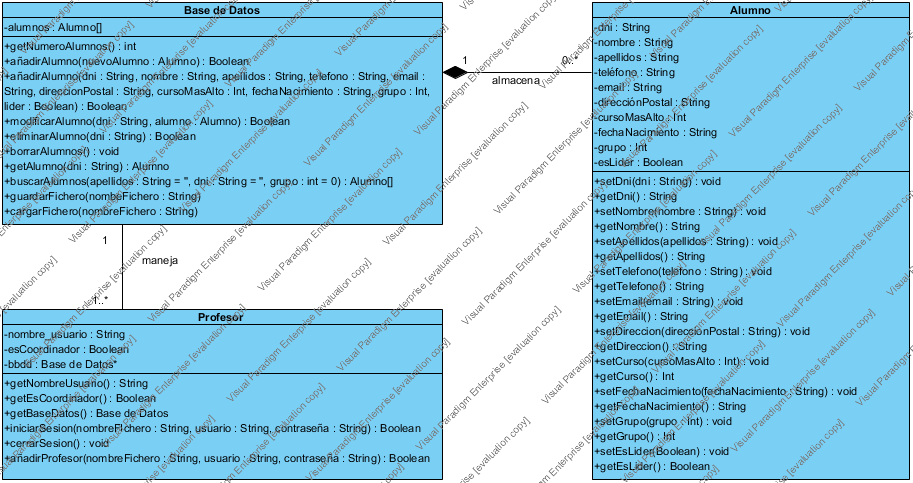
\includegraphics[width=1\textwidth]{../design/class_diagram}
	\caption{Diagrama de clases}
	\label{fig:class_diagram}
\end{figure}

\newpage
\section{Diagramas de secuencia}
El análisis de comportamiento se basará en los casos de uso previamente especificados y para
llevarlo a cabo se seguirá la metodología UML utilizando para ello la técnica de diagramas de
secuencias.

\subsection{Diagrama de secuencia. Añadir alumno}
\begin{figure}[h!]
	\centering
	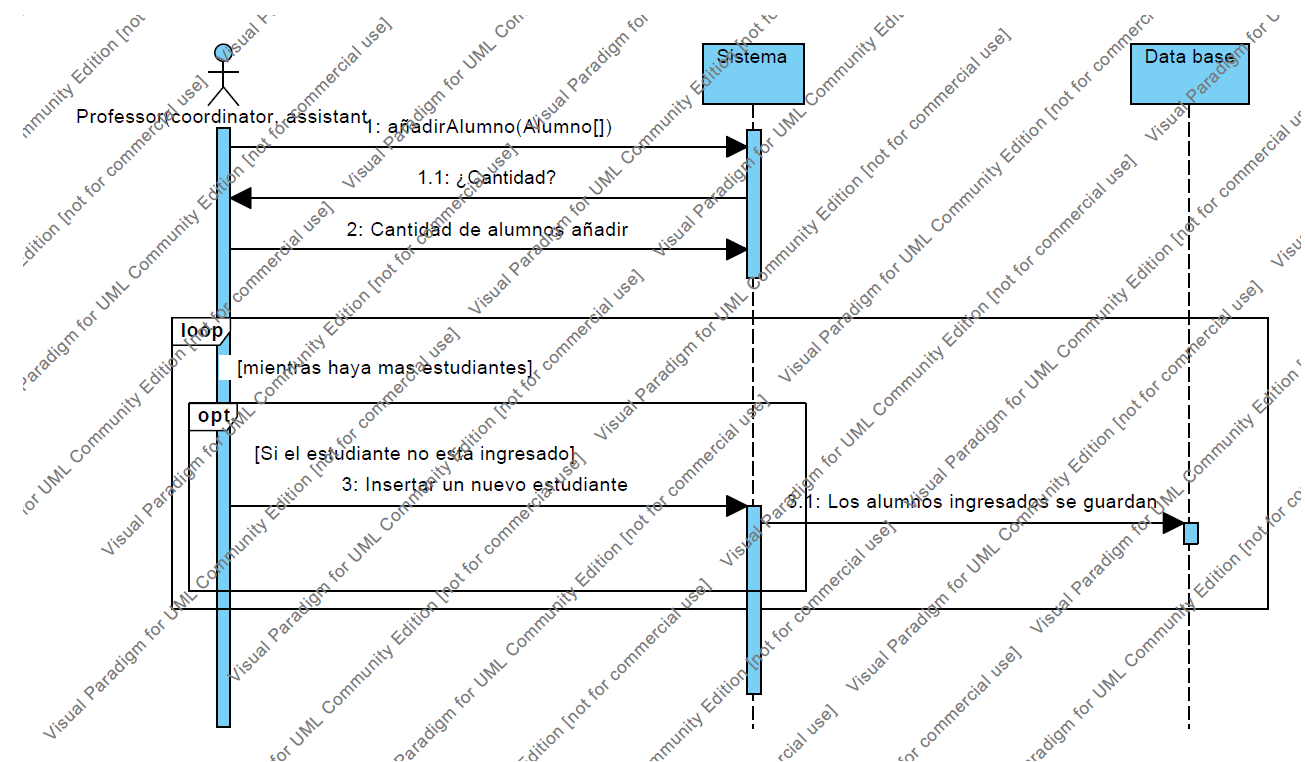
\includegraphics[width=1\textwidth]{../design/sd-1}
	\caption{Diagrama de secuencia del CU-1: Añadir alumno}
	\label{fig:sd001}
\end{figure}

\newpage
\subsection{Diagrama de secuencia. Modificar alumno}
\begin{figure}[h!]
	\centering
	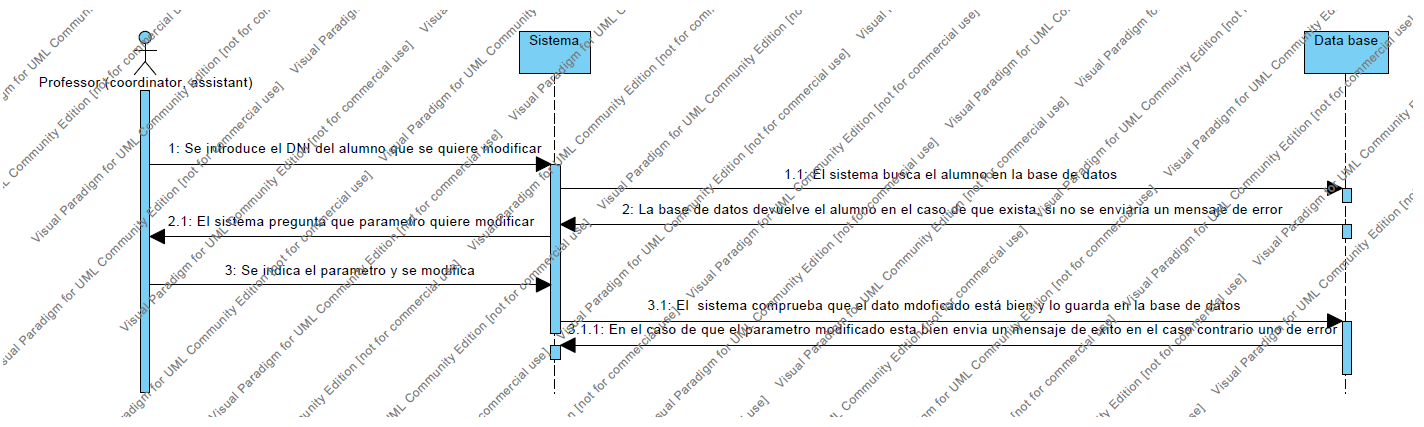
\includegraphics[width=1\textwidth]{../design/sd-2}
	\caption{Diagrama de secuencia del CU-2: Modificar alumno}
	\label{fig:sd002}
\end{figure}

\subsection{Diagrama de secuencia. Eliminar alumno}
\begin{figure}[h!]
	\centering
	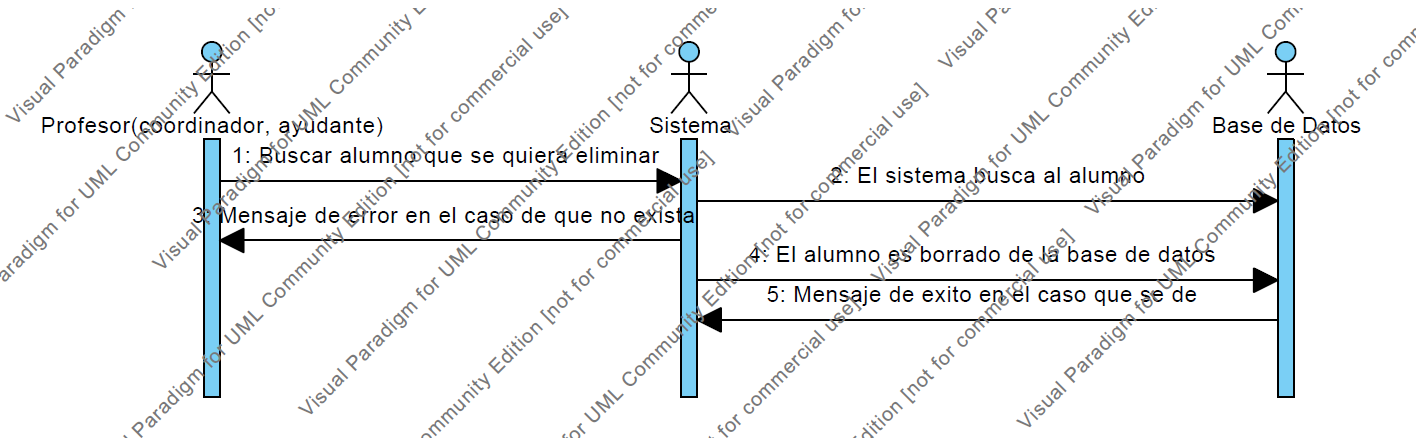
\includegraphics[width=1\textwidth]{../design/sd-3}
	\caption{Diagrama de secuencia del CU-3: Eliminar alumno}
	\label{fig:sd003}
\end{figure}

\newpage
\subsection{Diagrama de secuencia. Buscar alumnos}
\begin{figure}[h!]
	\centering
	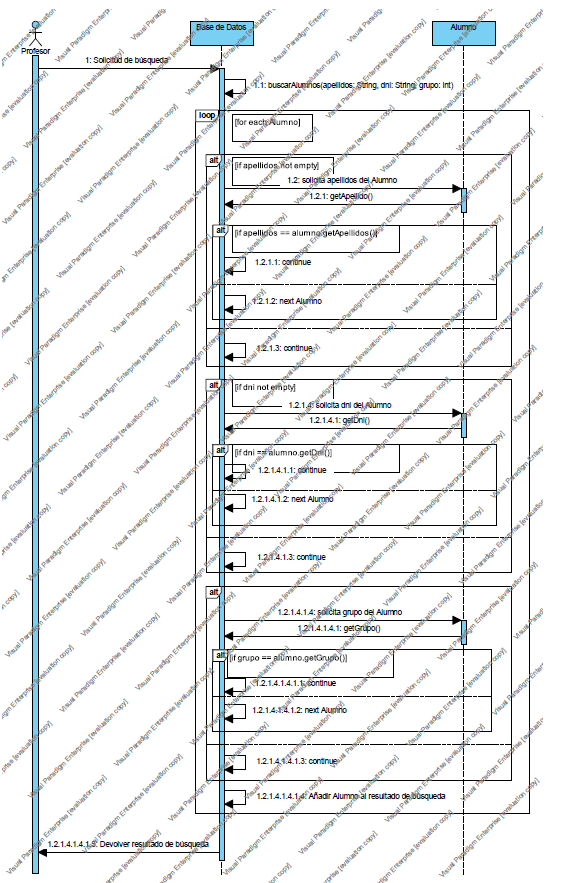
\includegraphics[width=0.75\textwidth]{../design/sd-4}
	\caption{Diagrama de secuencia del CU-4: Buscar alumnos}
	\label{fig:sd004}
\end{figure}

\newpage
\subsection{Diagrama de secuencia. Mostrar alumnos}
\begin{figure}[h!]
	\centering
	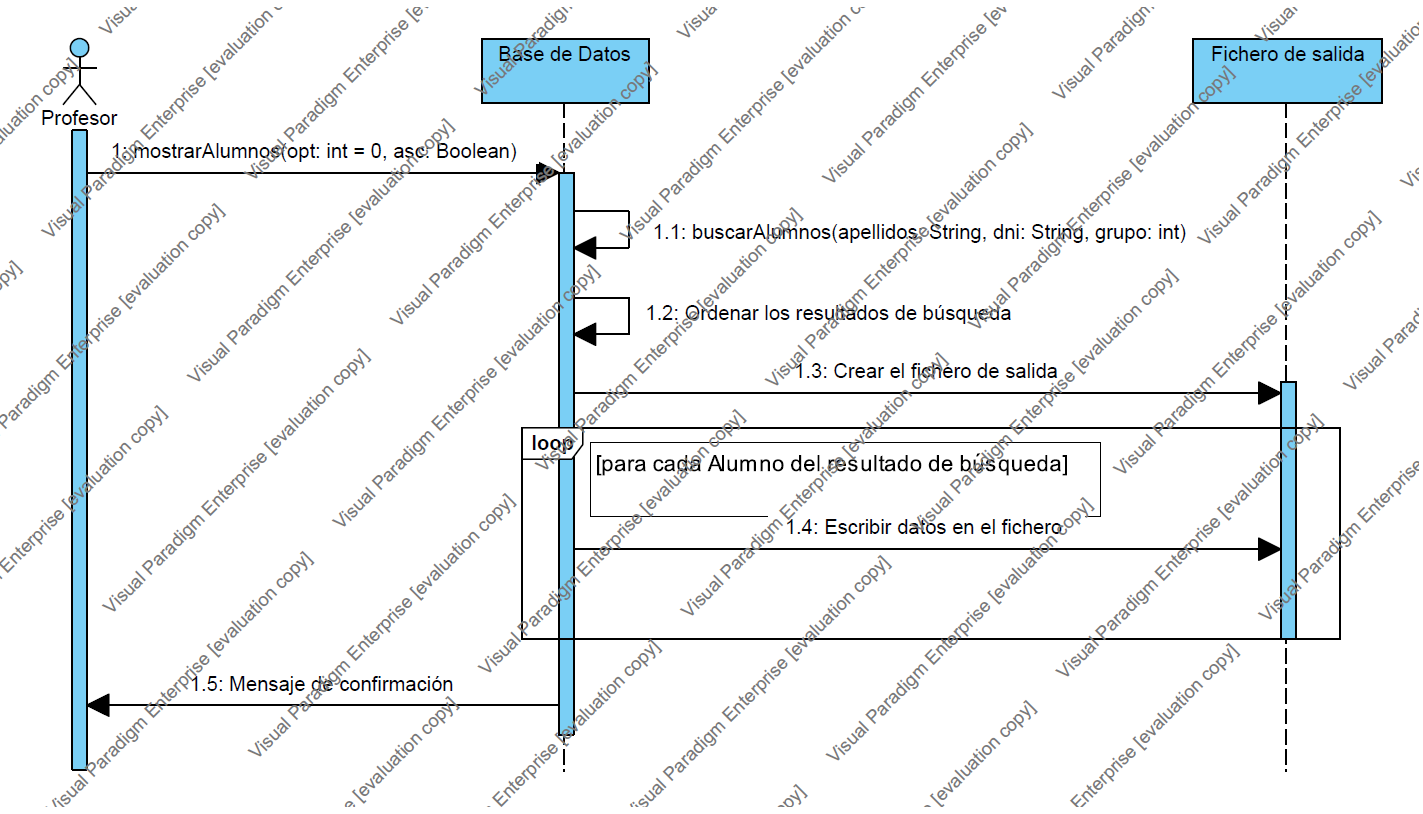
\includegraphics[width=1\textwidth]{../design/sd-5}
	\caption{Diagrama de secuencia del CU-5: Mostrar alumnos}
	\label{fig:sd005}
\end{figure}

\newpage
\subsection{Diagrama de secuencia. Guardar fichero}
\begin{figure}[h!]
	\centering
	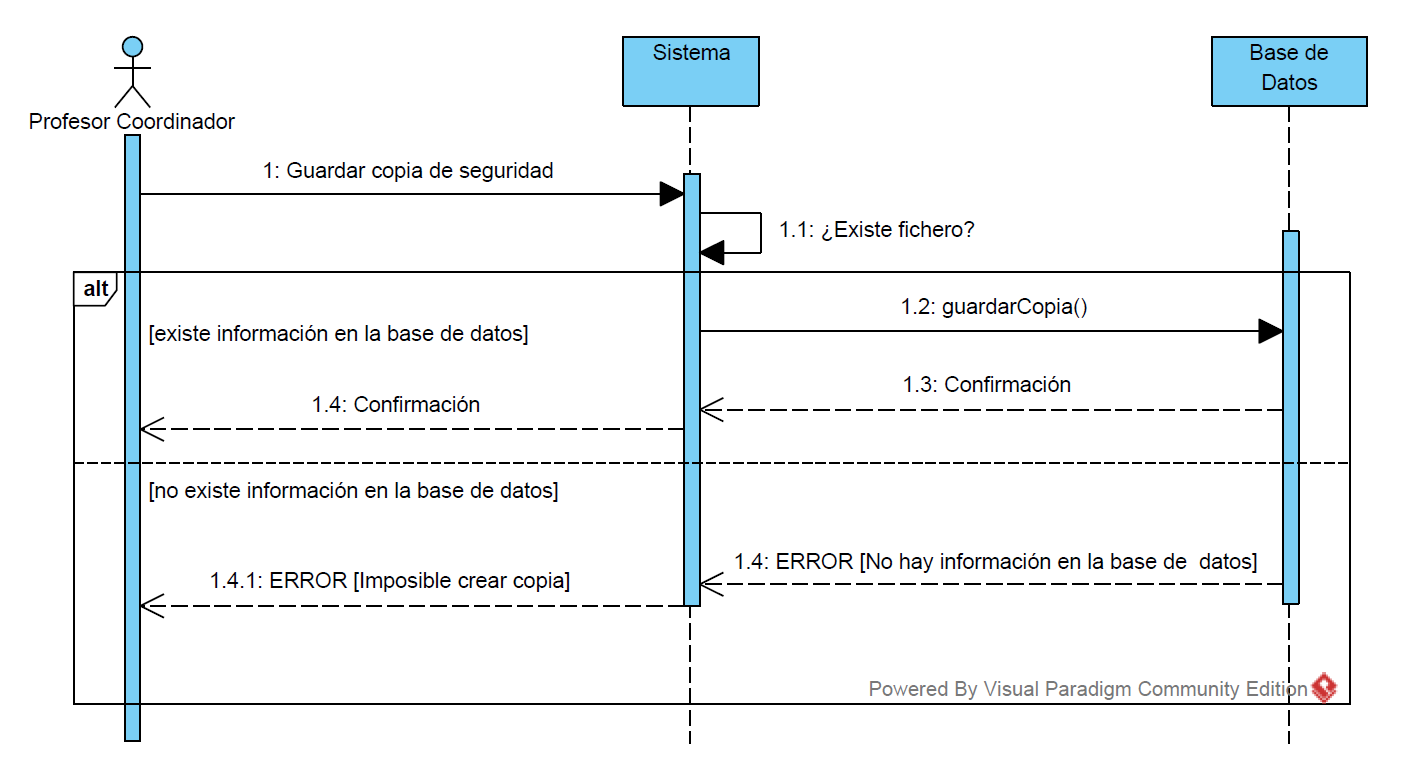
\includegraphics[width=0.9\textwidth]{../design/sd-6}
	\caption{Diagrama de secuencia del CU-6: Guardar fichero}
	\label{fig:sd006}
\end{figure}

\subsection{Diagrama de secuencia. Cargar fichero}
\begin{figure}[h!]
	\centering
	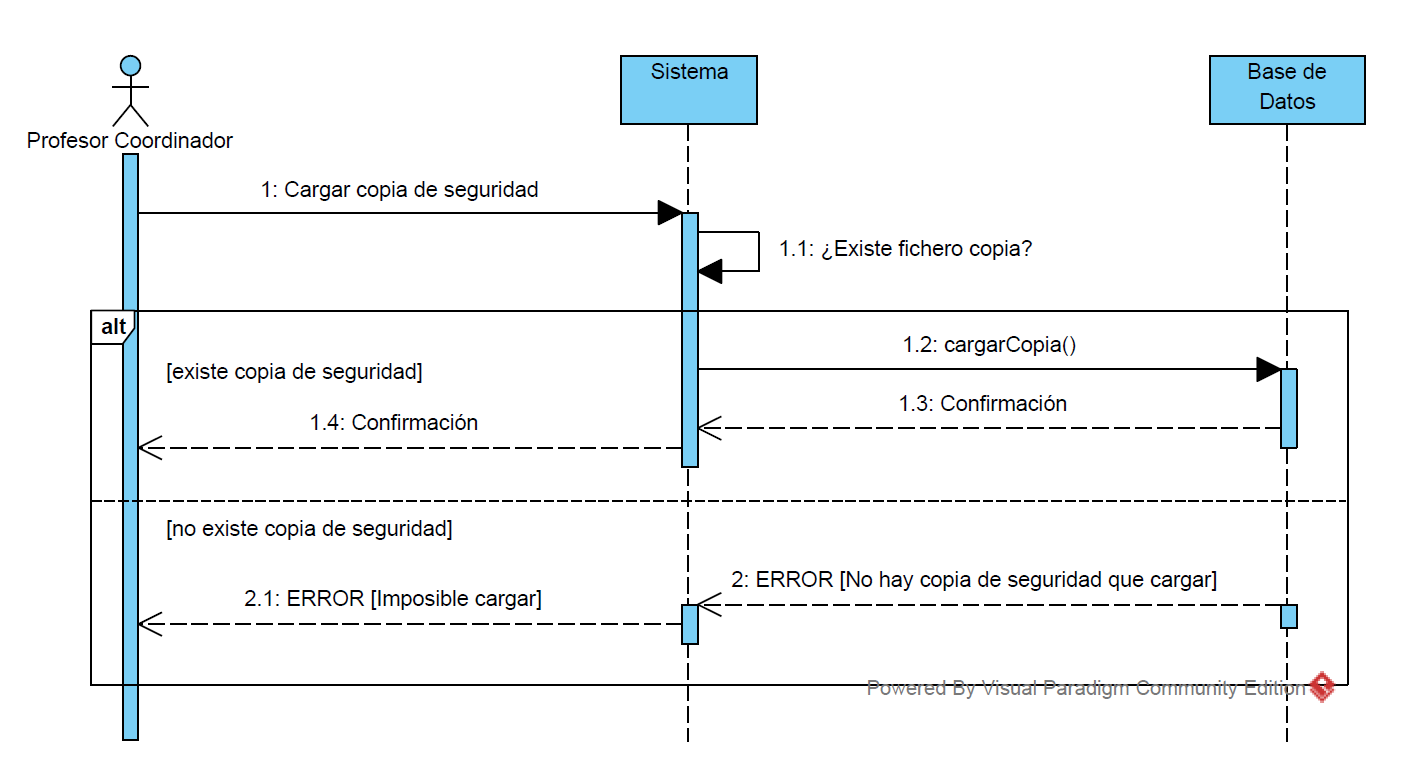
\includegraphics[width=0.9\textwidth]{../design/sd-7}
	\caption{Diagrama de secuencia del CU-7: Cargar fichero}
	\label{fig:sd007}
\end{figure}

\newpage
\subsection{Diagrama de secuencia. Identificar profesor}
\begin{figure}[h!]
	\centering
	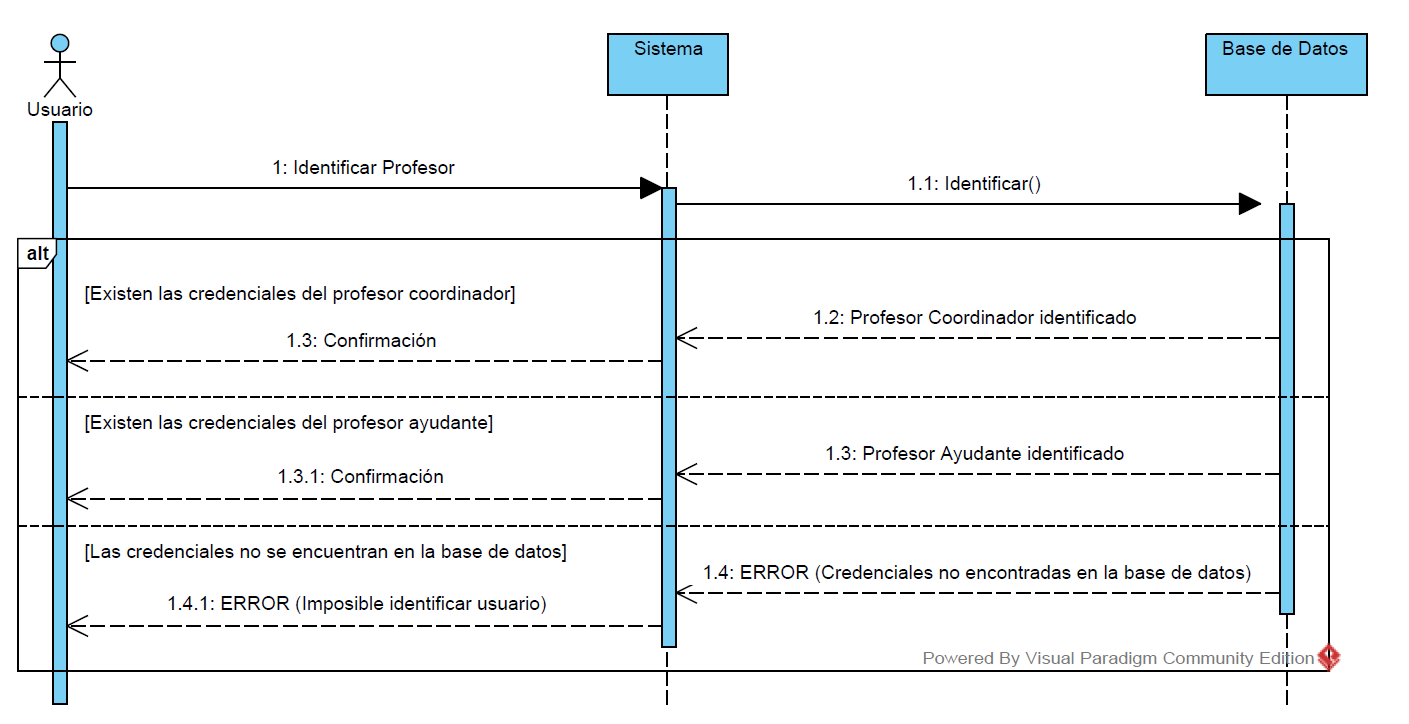
\includegraphics[width=1\textwidth]{../design/sd-8}
	\caption{Diagrama de secuencia del CU-8: Identificar profesor}
	\label{fig:sd008}
\end{figure}

\subsection{Diagrama de secuencia. Añadir profesor}
\begin{figure}[h!]
	\centering
	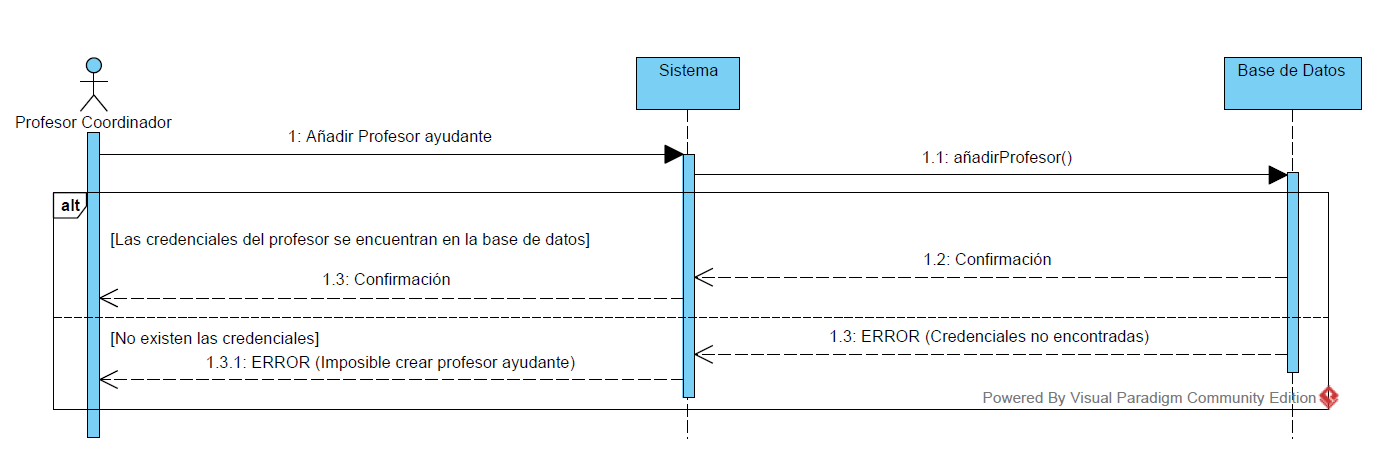
\includegraphics[width=1\textwidth]{../design/sd-9}
	\caption{Diagrama de secuencia del CU-9: Añadir profesor}
	\label{fig:sd009}
\end{figure}
\chapter{Implementación y pruebas}
\section{SCRUM}
\subsection{Product Backlog}
\begin{table}[h!]
	\centering
	\begin{tabular}{lcc}
		\toprule
		\textbf{Historia de Usuario} & \textbf{Estimación} & \textbf{Prioridad} \\
		\midrule
		Como usuario quiero poder identificarme en el sistema.	& 2	& 1 \\
		Como usuario quiero poder añadir otros usuarios en el sistema. & 2 &2 \\
		Como usuario quiero poder añadir alumnos al listado. & 1 & 3 \\
		Como usuario quiero poder buscar y seleccionar alumnos entre el listado. & 1 & 4 \\
		Como usuario quiero poder visualizar un listado de alumnos. & 3 & 5 \\
		Como usuario me interesa poder guardar los datos almacenados externamente. & 2 &6 \\
		Como usuario me interesa poder cargar los datos almacenados externamente. & 2 & 7 \\
		Como usuario quiero poder modificar alumnos del listado. &	1&	8 \\
		Como usuario quiero poder eliminar alumnos del listado.	 & 1 &	9 \\
		\bottomrule
\end{tabular}
\caption{\label{tab:product_backlog}Product Backlog}
\end{table}

\newpage
\subsection{Sprint Backlog}
\begin{table}[h!]
	\centering
	\begin{tabular}{cccccc}
		\toprule
		\textbf{Tarea} & \textbf{Quién} & \textbf{Estado} & \textbf{Semana 1} & \textbf{Semana 2} & \textbf{Semana 3} \\
		\midrule
		HU008.	& i72pehej & Terminada & 0.5 & 0.5 & 0 \\
		HU009.	& i72pehej & Terminada & 0.5 & 0.5 & 0 \\
		HU001.	& i72orled & Terminada & 0.5 & 0 & 0 \\
		HU004.	& i42semoa & Terminada & 0.5 & 0 & 0 \\
		HU005.	& i42semoa & Terminada & 4 & 2 & 0 \\
		HU006.	& i72pehej & Terminada & 2 & 1 & 0 \\
		HU007.	& i72pehej & Terminada & 2 & 1 & 0 \\
		HU002.	& i72orled & Terminada & 1 & 0.5 & 0 \\
		HU003.	& i72orled & Terminada & 1 & 0 & 0 \\
		\bottomrule
\end{tabular}
\caption{\label{tab:sprint_backlog}Sprint Backlog}
\end{table}

\subsection{Burndown Chart}
\begin{figure}[h!]
	\centering
	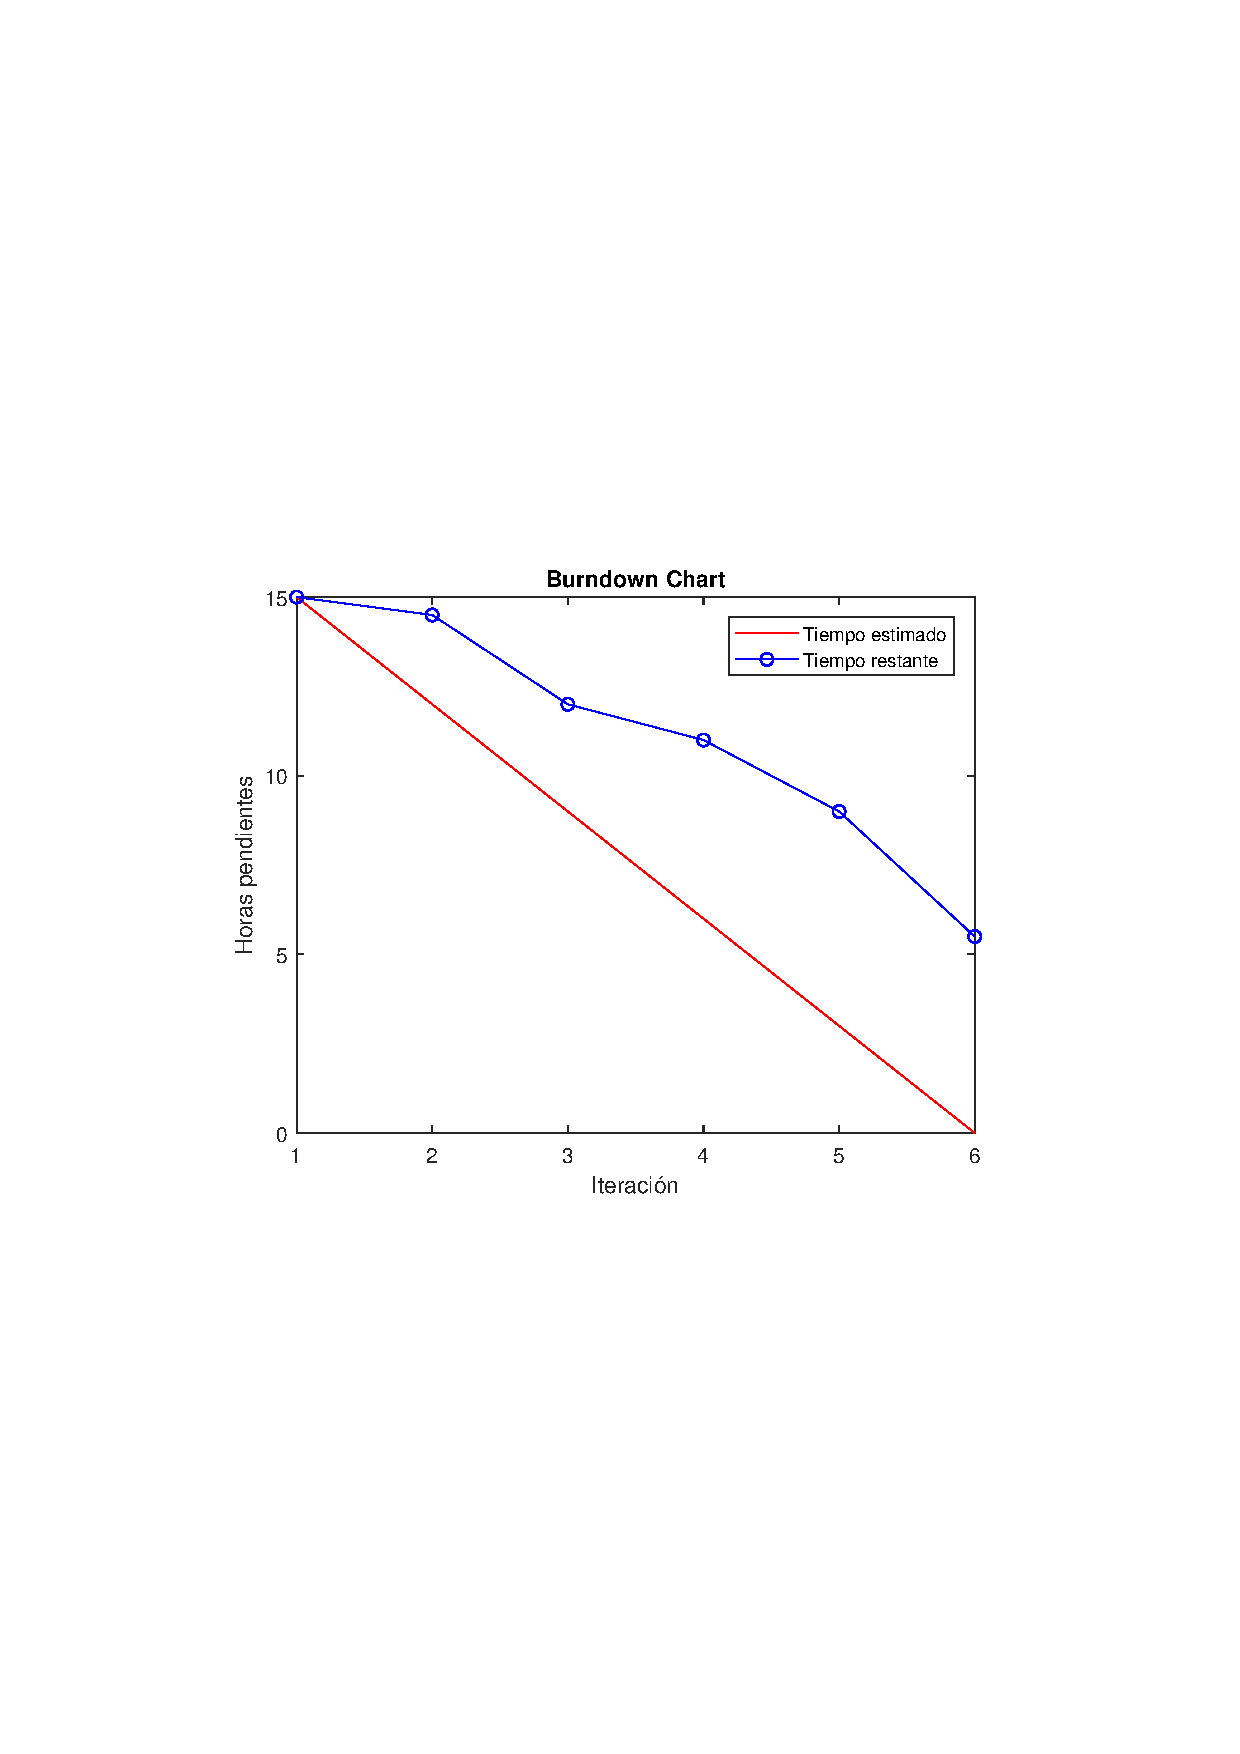
\includegraphics[width=0.85\textwidth]{burndown_chart}
	\caption{Burndown chart}
	\label{fig:burndown_chart}
\end{figure}

\newpage
\section{Código}
\subsection{alumno} \label{alumno}
\lstinputlisting{../code/alumno.hpp}
\lstinputlisting{../code/alumno.cpp}

\newpage
\subsection{baseDatos} \label{baseDatos}
\lstinputlisting{../code/basedatos.hpp}
\lstinputlisting{../code/basedatos.cpp}

\newpage
\subsection{profesor} \label{profesor}
\lstinputlisting{../code/profesor.hpp}
\lstinputlisting{../code/profesor.cpp}

\newpage
\subsection{is} \label{is}
\lstinputlisting{../code/is.hpp}

\newpage
\subsection{ppal-is} \label{ppal-is}
\lstinputlisting{../code/ppal-is.cpp}

\newpage
\section{Técnicas de validación}
En este capítulo se llevarán a cabo una serie de técnicas de validación para comprobar la corrección y completitud de la información, realizando para ello distintas matrices de validación.

\subsection{Matriz de correspondencia RF/Casos de Uso}
En la tabla \ref{tab:correspondencia_rf_cu} se muestra la matriz de correspondencia entre los requisitos funcionales y los casos de uso.

\begin{table}[h!]
	\centering
	\begin{tabular}{cccccccccc}
		\toprule
		& CU-1 & CU-2 & CU-3 & CU-4 & CU-5 & CU-6 & CU-7 & CU-8 & CU-9  \\
		\midrule
		RU-1 &  x&&&&&&&&   \\
		RU-2 &  &x&&&&&&&\\
		RU-3 &  &&x&&&&&&\\
		RU-4 &  &&&x&&&&&\\
		RF-5 &  &&&&x&&&&\\
		RF 6 &  &&&&&x&&&\\
		RU-7 &  &&&&&&x&&\\
		RU-8 &  &&&&&&&x&\\
		RU-9 &  &&&&&&&&x\\
		\bottomrule
	\end{tabular}
	\caption{\label{tab:correspondencia_rf_cu}Matriz de correspondencia RF/Casos de Uso}
\end{table}

\subsection{Matriz de correspondencia CU/Clases}
En la tabla \ref{tab:correspondencia_cu_clases} se muestra la matriz de correspondencia entre los casos de uso y las clases.
\begin{table}[h!]
	\centering
	\begin{tabular}{cccc}
		\toprule
			   & Alumno & BaseDatos & Profesor \\
		\midrule
		CU-1   & x       & x        &       \\
		CU-2   & x       & x        &       \\ 
		CU-3   & x       & x        &       \\
		CU-4   & x       & x        &       \\
		CU-5   & x       & x        &       \\
		CU-6   & x       & x        &       \\
		CU-7   & x       & x        &       \\ 
		CU-8   &         &          & x     \\
		CU-9   &         &          & x     \\
		\bottomrule
	\end{tabular}
	\caption{\label{tab:correspondencia_cu_clases}Matriz de correspondencia CU/Clases}
\end{table}

\end{document}